\begin{figure*}[!hb]
    \centering
    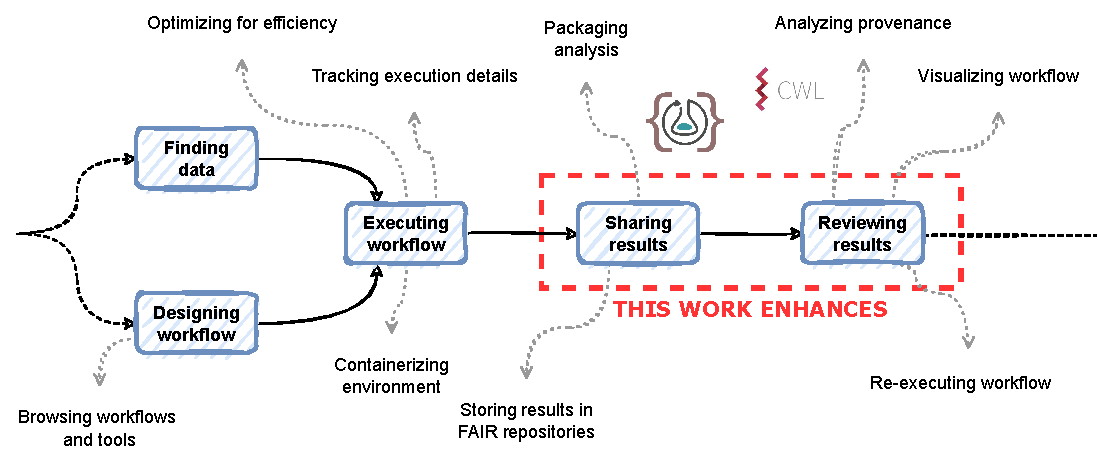
\includegraphics[width=1\textwidth]{background/vision.pdf}
    \caption{A vision of an ecosystem of workflow-related resources and its benefits for the reproducibility of computational processes. In this vision, workflows and data are stored in FAIR repositories, are executed in containerized environments by workflow systems which leverage efficient job-scheduling technologies and track details of the computation.  
    After publication, the results of the workflow can be analyzed, and workflows can optionally be re-executed as the start of new projects which build upon the research. 
    Fundamental to the success of this approach is the interoperability of the components of the ecosystem. In this work, we focus on workflow-centric Research Objects as a common format for the sharing and analysis of computational results.
    %\todorenske{Keep CWL(Prov) and ROCrate logos in?}
    }
    \label{fig:vision}
\end{figure*}